\documentclass[a4paper]{article}

\usepackage[utf8]{inputenc}
\usepackage[top=20pt, bottom=20pt, left=20pt, right=20pt]{geometry}
\usepackage{graphicx}


\title{UML2Java V1.0}
\author{D. Mal\'{y} \, S.Sherar\, L.Smith\\Aberystwyth University}
\date{}


\begin{document}
\maketitle
\tableofcontents
\section{File Menu}
\subsection{Create new Class Diagram}
To create a new Class Diagram, go to the top menu bar and press \texttt{File $\rightarrow$ New}

\begin{center} 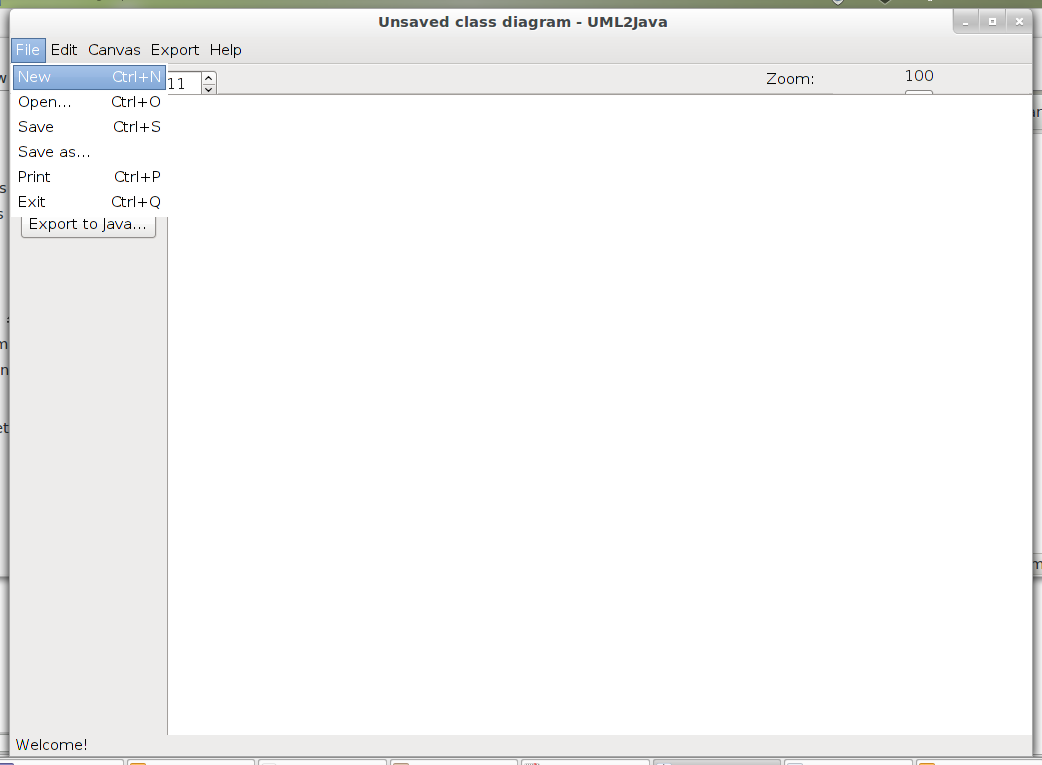
\includegraphics[scale=0.4]{./images/file-new.png} \end{center}
\subsection{Open an existing diagram}
To open a previously saved diagram, go to the top menu bar and press \texttt{File $\rightarrow$ Open...} or simply press \texttt{CTRL+O}
This will open up a new window asking for the location of the file you wish to open
%insert open document image
\subsection{Saving a diagram}
To save a diagram, go to the top menu bar and press File $\rightarrow$ Save or simply press \texttt{CTRL+S}
%insert save document image


\end{document}
